% !TeX root = ../../../main.tex
\begin{figure}[!htp]
\ChThreeFloatContents
  {ch03:fig:graphical_ATE_trend}
  {\caption{Estimated Average Treatment Effect (ATE) of non-adherence across time snapshots \(\tau\) for different survival models. Each panel corresponds to a specific survival model (CoxPH, Random Survival Forest, DeepSurv, and DeepHit), with ATE estimates reported for multiple meta-learning approaches (T-learner, S-learner, and Matching). The Causal Survival Forest (CSF) is included in all plots as a baseline for comparison. Shaded regions represent standard deviations, illustrating the uncertainty in the estimates.}}
  {%
    \subfigure[CoxPH]{\label{ch03:fig:graphical_ate_coxph}%
      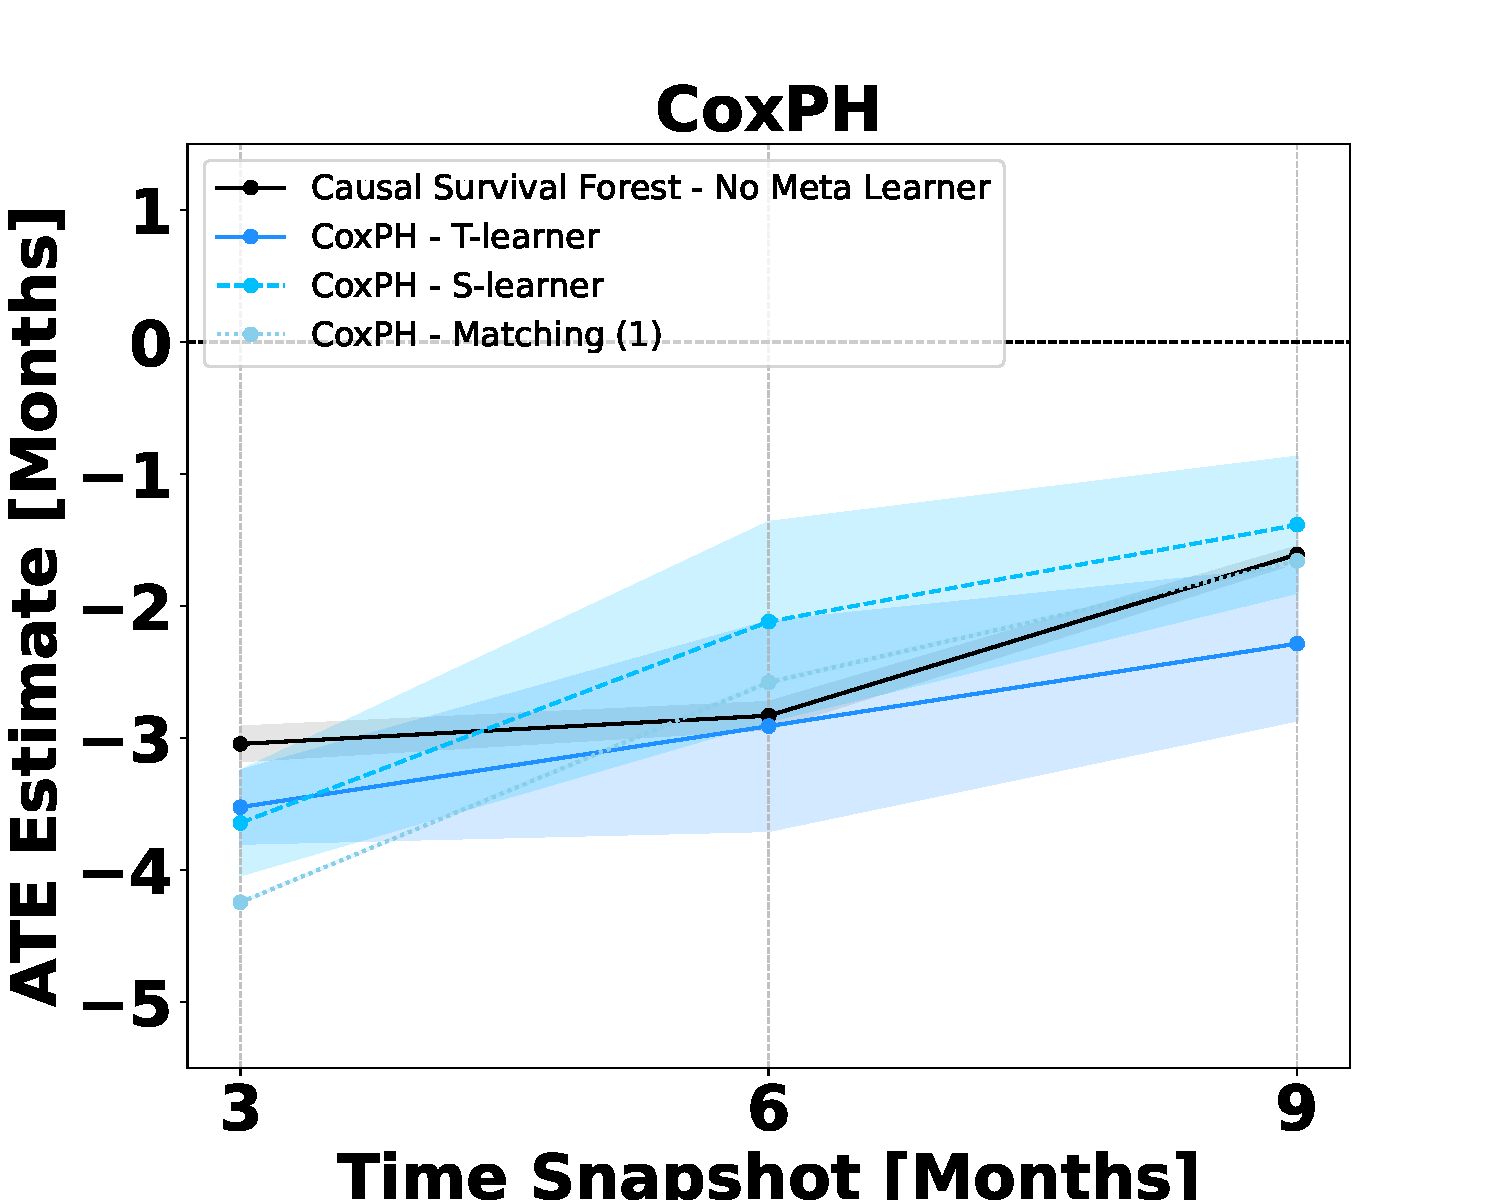
\includegraphics[width=.45\linewidth]{Appendices/appendix-ch03/images/Graphical_ATE/Graphical_ATE_CoxPH.pdf}}%
    \subfigure[RandomSurvivalForest]{\label{ch03:fig:graphical_ate_rsf}%
      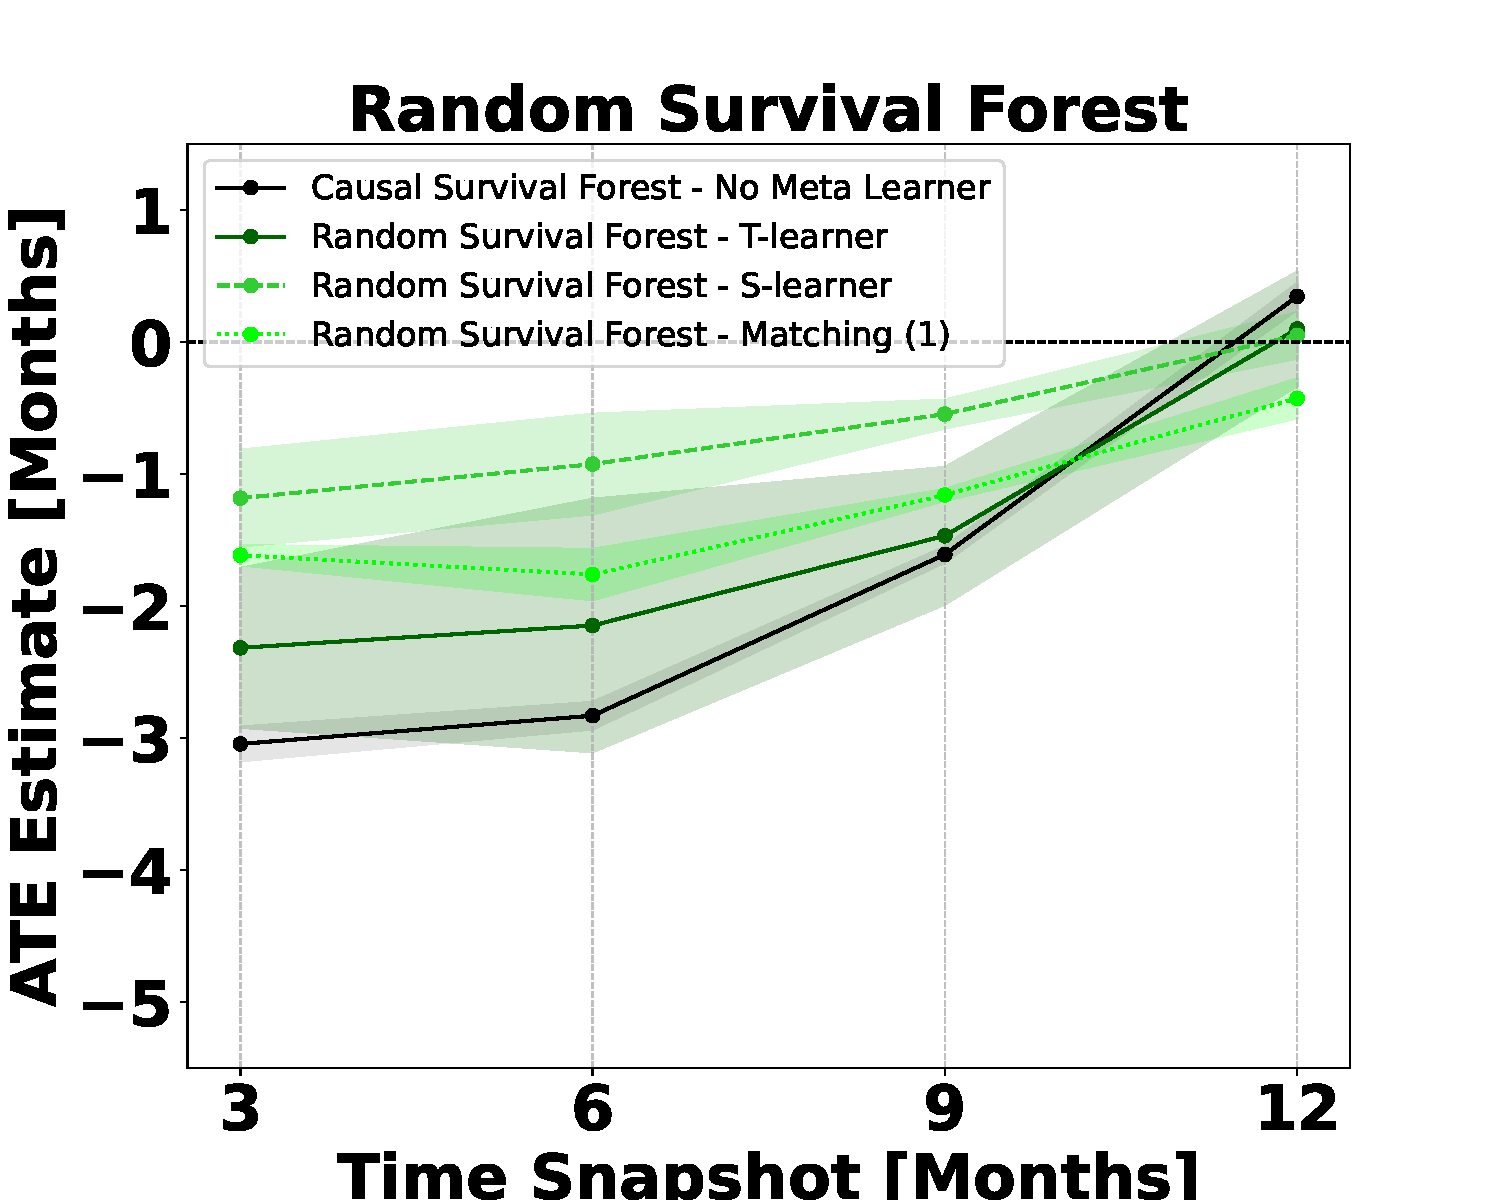
\includegraphics[width=.45\linewidth]{Appendices/appendix-ch03/images/Graphical_ATE/Graphical_ATE_Random_Survival_Forest.pdf}}%
      \\
    \subfigure[DeepSurv]{\label{ch03:fig:graphical_ate_deepsurv}%
      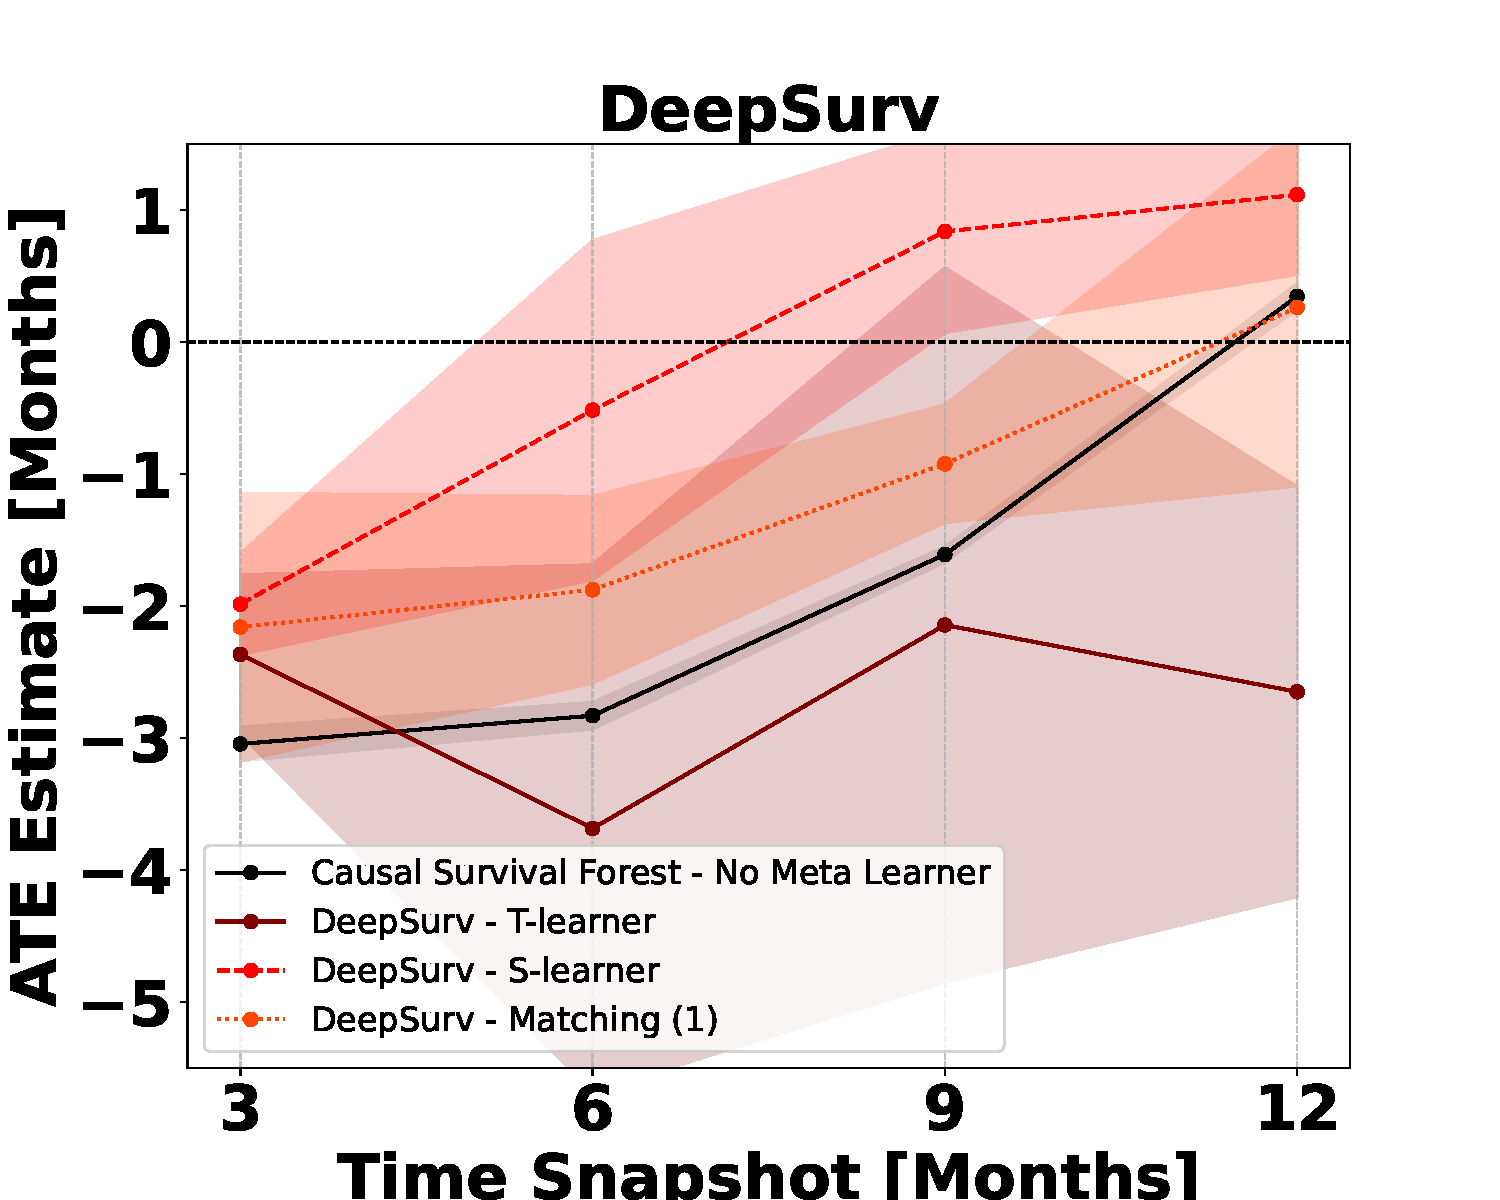
\includegraphics[width=.45\linewidth]{Appendices/appendix-ch03/images/Graphical_ATE/Graphical_ATE_DeepSurv.pdf}}%
    \subfigure[DeepHit]{\label{ch03:fig:graphical_ate_deephit}%
      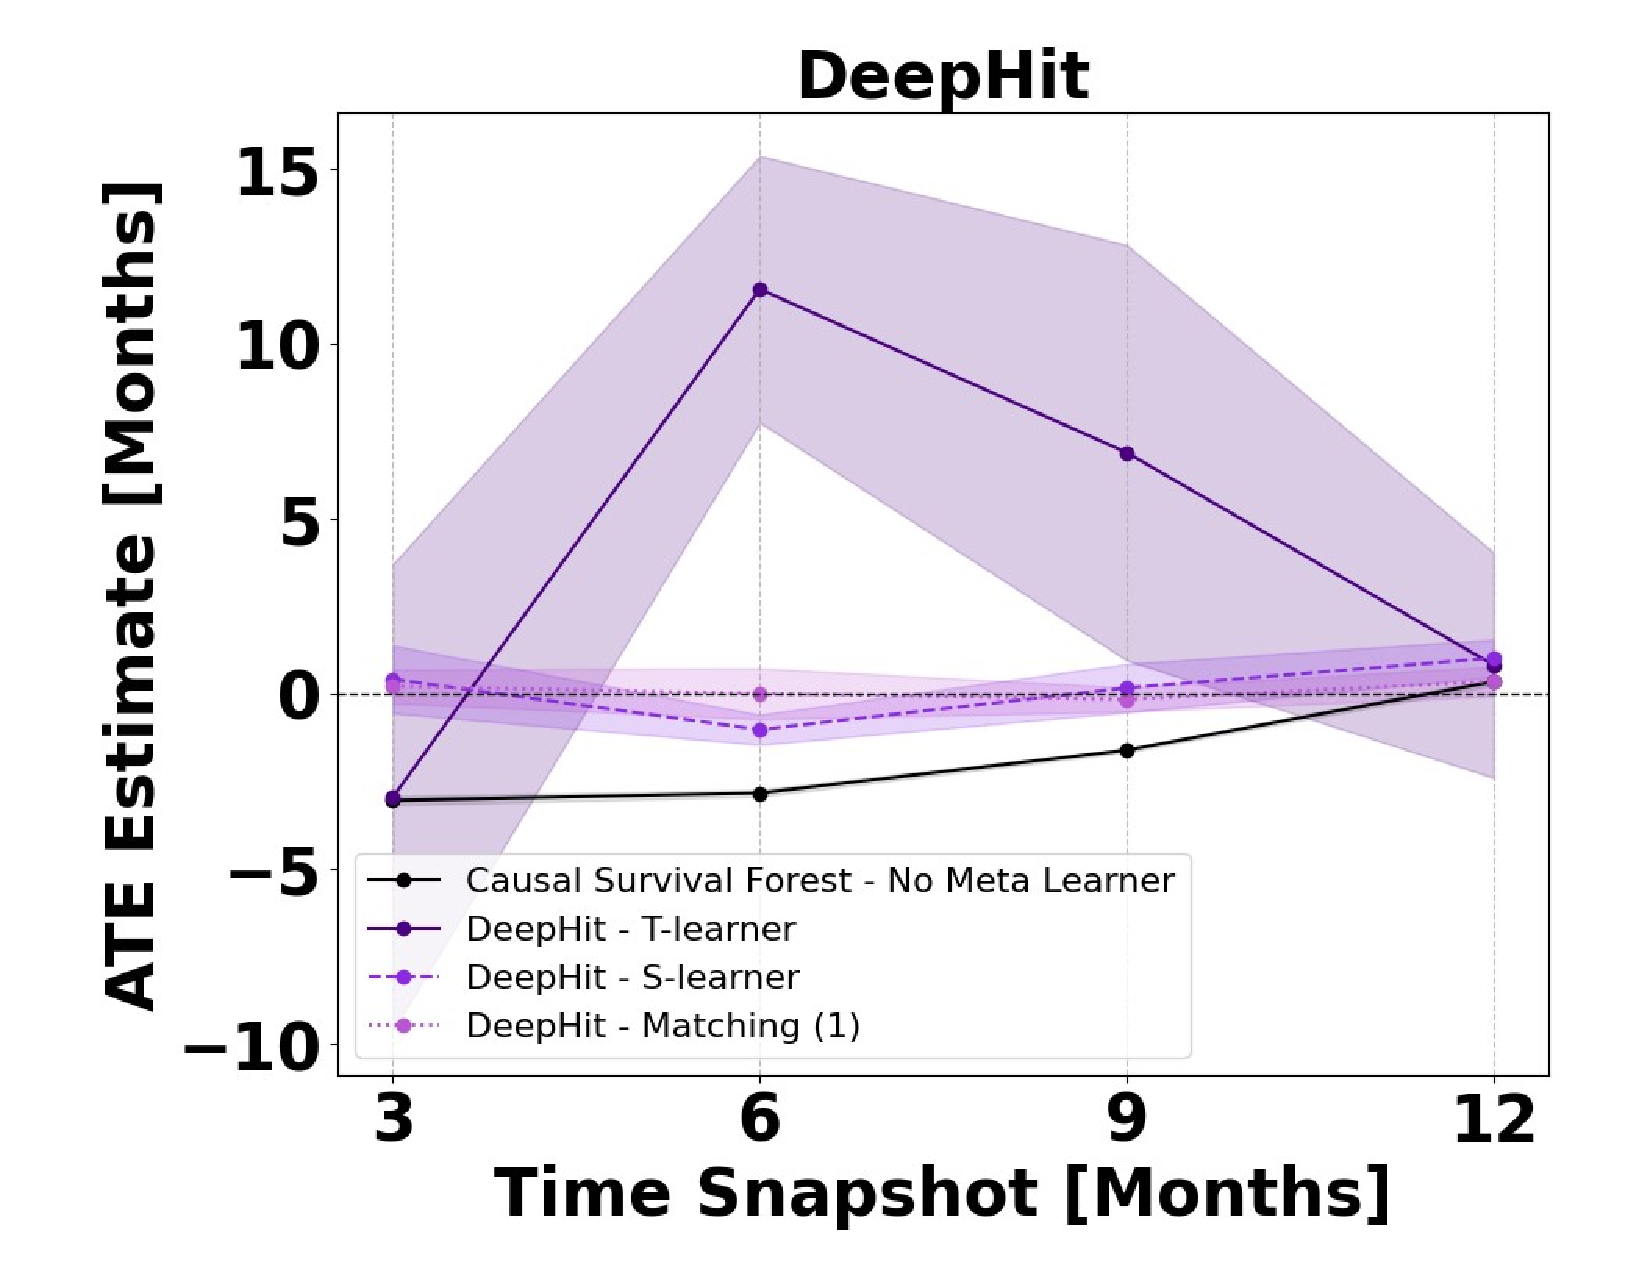
\includegraphics[width=.46\linewidth]{Appendices/appendix-ch03/images/Graphical_ATE/Graphical_ATE_DeepHit.pdf}}%
  }
\end{figure}